\section{X-ray computed tomography}
One step up from basic radiography is computed (axial) tomography (CT, formerly
CAT). The goal here is to create image slices of patients in the cross-sectional
plane rather than the frontal plane (tomography is Greek for ``slice writing'').
To accomplish this, the X-ray source-detector pair is rotated around the
patient. From this raw data, a so-called filtered back projection algorithm can
reconstruct the whole cross section image. A computer is needed to make sense of
the output, hence the \emph{computed} in the name. \autoref{fig:ctscan} shows an
example of a chest CT scan and \autoref{fig:ctscanner} shows an actual scanner.

\begin{figure}[ht]
\begin{center}
  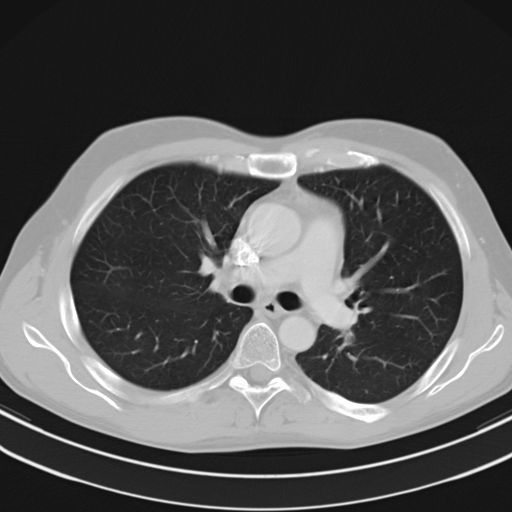
\includegraphics[width=0.4\linewidth]{img/ct-thorax.jpg}
  \caption{Example of a thoracic CT scan. The heart is clearly visible in the
  center. Bones (ribs, sternum, spine) are also easy to spot in the periphery.
  The large black area represents the lungs filled with air.}
  \label{fig:ctscan}
\end{center}
\end{figure}

\subsection{History}
Before computed tomography became possible, some simpler techniques were already
being used to obtain slices from inside the patient's body. These techniques
were called (non-computed) tomography. One example is linear tomography,
where source and detector move on parallel tracks, but in opposite directions,
during the scanning process. This way, one section of the patient is always
projected on the same spot of the detector, while the rest is averaged out.
Obviously, these techniques where nowhere near as accurate as the CT scanners we
know today.

In 1917, Johann Radon - an Austrian mathematician - presented the first
algorithm to reconstruct a function from its projections: the Radon transform
\cite{radon}.

After World War II, the development of computers gained momentum, but it would
still take a long while before the ``computed" in ``computed tomography" became
feasible. In the 1960's, the South African Allan McLeod Cormack continued
working on the mathematics invented by Radon \cite{ctreview}. A decade later, in
1972, the first operational brain CT scanner (the EMI scanner) was designed by
Godfrey Hounsfield, an Englishman. A scan took about 5 minutes, after which a
computer performed calculation for up to 150 minutes. The final output was a
80px $\times$ 80px image. Cormack and Hounsfield shared the 1979 Nobel Prize in
Physiology or Medicine for their work related to CT scans \cite{ctbook}.

\begin{figure}[ht]
\begin{center}
  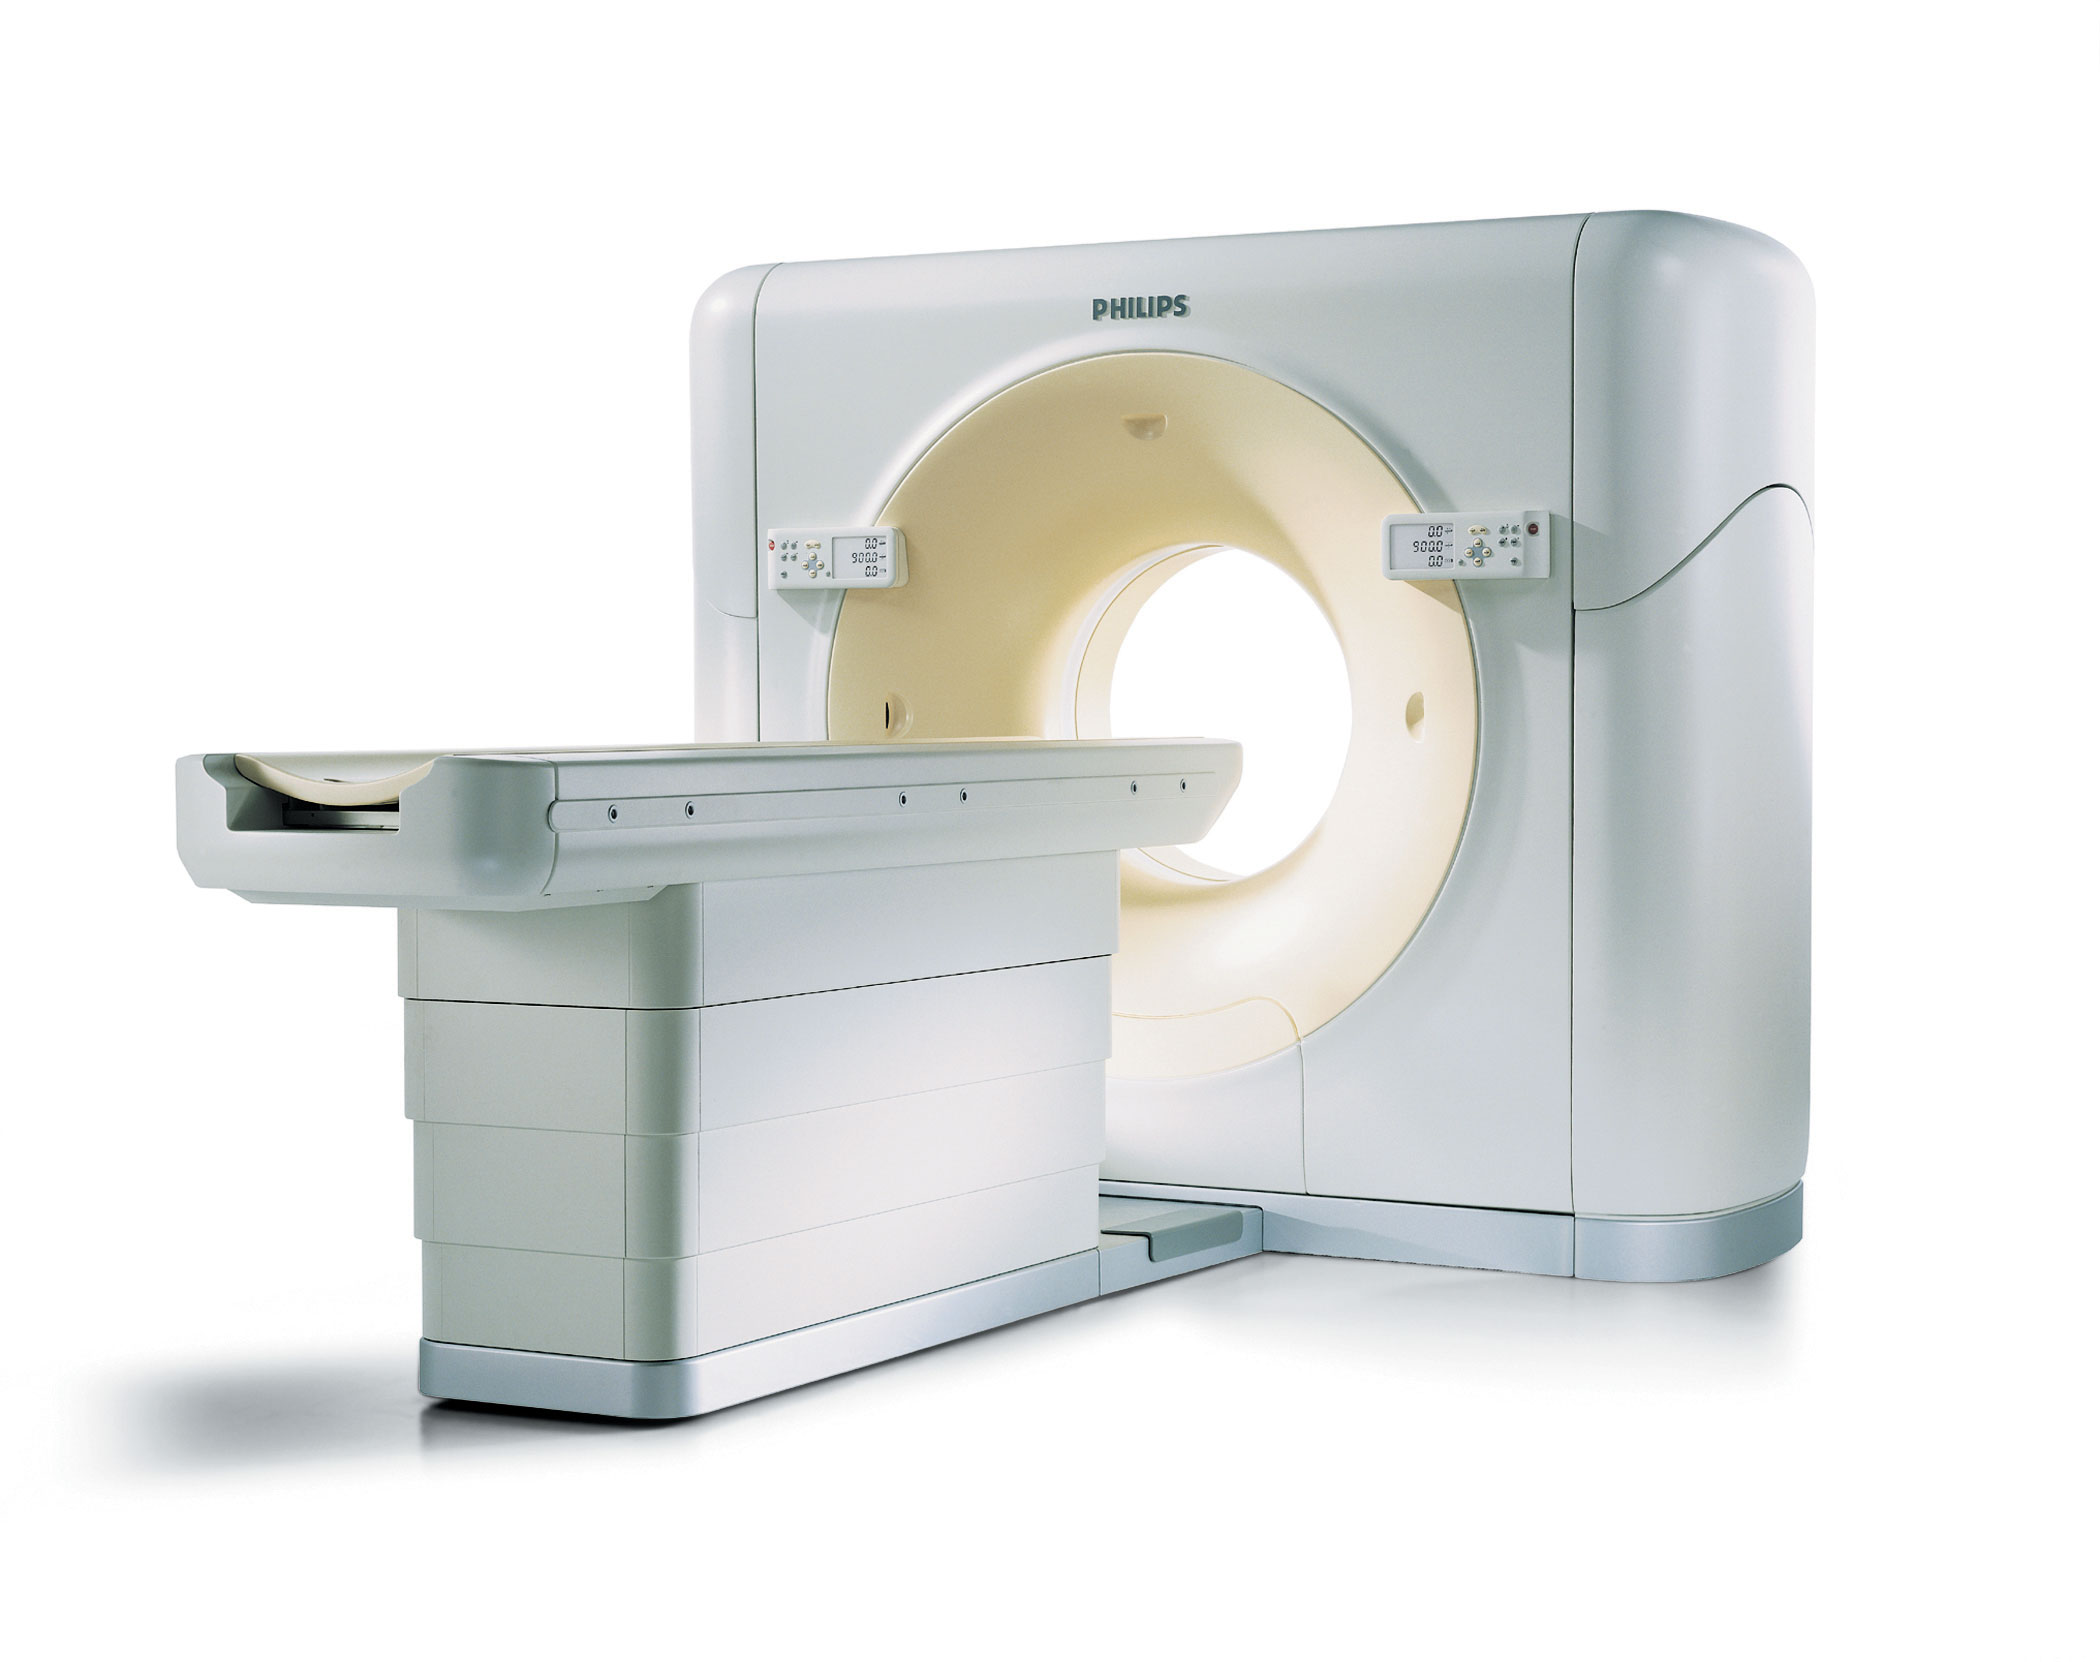
\includegraphics[width=\linewidth]{img/ctscanner.jpg}
  \caption{A CT scanner made by Philips. The patient takes place on the table
  and slowly slides through the toroid wherein the rotating X-ray
  source-detector pair is embedded.}
  \label{fig:ctscanner}
\end{center}
\end{figure}

\subsection{Technical background}
Just like radiographs, CT scanners are based on X-ray technology. They also
require a source and a detector, but this time they can rotate along the
patient. For every rotation angle $\theta$, we obtain an intensity profile
$I_\theta(r)$ along the axis $r$ perpendicular to the incoming X-rays (with
uniform incoming intensity $I_0$). The family of functions $I_\theta$ can be
transformed into an attenuation profile $p(r, \theta) = -\ln \tfrac{I_\theta(r)}{I_0}$
(often called a sinogram). This $p(r, \theta)$ is called the Radon transform of
the attenuation distribution $\mu(x,y)$ in the slice plane.
\begin{equation}
	p(r, \theta) = \mathscr{R}\{ \mu(x,y) \}
\end{equation}

In short, the projections $p$ is what we can measure (or at least sample at
fixed intervals) and the attenuation distribution $\mu$ is what we are
interested in. The mathematics required to go from the latter to the former are
pretty straightforward, but the reverse is more complicated. The inverse Radon
transform $\mu = \mathscr{R}^{-1}(p)$ is needed.

We will not go into details, but the solution lies in the projection theorem.
This theorem states that the 2D Fourier transform $M(k_x, k_y)$ of $\mu(x,y)$
is equal to the 1D Fourier transform $P(k, \theta)$ of $p(r, \theta)$ (save for
a simple polar coordinate transformation).

\begin{equation}
\mathscr{F}_{1D}\{ p(r, \theta) \} = P(k, \theta) = M(k \cos \theta, k \sin
\theta) = \mathscr{F}_{2D}\{ \mu(x, u) \}
\end{equation}

Because the inverse Fourier transform is well understood, we have a solution to
our problem. Simply calculate $P$ from $p$ as explained above, and then apply
the inverse 2D Fourier transform to obtain $\mu$. By using the polar version of
the Fourier transform, we can reduce artifacts. This approach is called filtered
back projection \cite{suetens}.

After all the calculations are performed, we typically acquire a 512px $\times$
512px scan. The values of the pixels in a CT scan are referred to as the CT
numbers and are expressed in Hounsfield Units (HU). They are calculated using
the fomula below, where $\mu$ is again the attenuation coefficient.
\begin{equation}
	\text{CT number} = \frac{\mu -
	\mu_{\text{H}_2\text{O}}}{\mu_{\text{H}_2\text{O}}} \cdot 1000
\end{equation}

From this, it becomes obvious that the CT number of air (with $\mu = 0$) is
-1000 HU and that the CT number of water is 0 HU. Bones on the other hand have a
very high attenuation coefficient and thus have a CT number in the thousands.
Soft tissue lies somewhere in between.

\subsection{Recent advancements}
The previous section assumed parallel X-ray beams. However, newer generation
scanners often employ cone-shaped beams. The procedure outlined above can
reconstruct a single slice by rotating around the subject by 180 degrees at a
time (a circular CT). On the other hand, modern CT scanners often spiral around
the patient while he moves through the toroid (a helical CT) to speed up the
process and thus decrease the exposure. Another useful trick is to capture
multiple slices at once by using multiple detector arrays. Until recently,
manufacturers were in a so-called \emph{slice wars} to offer the most detector
arrays. Needless to say, all this substantially complicates the mathematics
required to perform a back projection, but it is feasible and daily used in
hospitals around the world.

Another point of interest today is the combination of successive CT slices to
generate a 3D model of the patient. Because of advancements in computer
technology and algorithms, we can now post-process this 3D model to
automatically segment the organs and other structures. This can for example help
physicians plan their actions before and during complex surgery.

\subsection{Future expectations}
Because CT scanners still require relatively high doses of radiation, this is
not an ideal solution. MRI scanners offer a safer alternative, but the large
magnetic fields produced make them impossible to use on patients with ferromagnetic
implants. Another advantage over MRI is the superior sub-millimeter resolution
that only CT scanners can offer. These are only some of the reasons why they
will not be replaced anytime soon. Future research will attempt to make CT
scanners even faster and allow them to produce clearer (i.e., higher contrast)
images with lower doses.